%-- coding: UTF-8 --
\documentclass[12pt]{ctexart}

%\usepackage[UTF8]{ctex}
\usepackage{geometry}
\geometry{a4paper,scale=0.8}

\date{} %2020-09-15
\usepackage[algo2e, linesnumbered,ruled,lined]{algorithm2e}
\usepackage{algpseudocode}  
\usepackage{amsmath}
\usepackage{amssymb}
\usepackage{graphicx}
\usepackage{float}
 \usepackage{natbib}
\usepackage{graphicx}
\usepackage{color}
\usepackage{algorithm}  
\usepackage{subfigure}
\usepackage{outlines}
\usepackage{ulem}
\usepackage{listings}
\usepackage{color}
\usepackage[T1]{fontenc}
\usepackage[utf8]{inputenc}
\usepackage{tabularx,ragged2e,booktabs,caption}
\newcolumntype{C}[1]{>{\Centering}m{#1}}
\renewcommand\tabularxcolumn[1]{C{#1}}

\definecolor{dkgreen}{rgb}{0,0.6,0}
\definecolor{gray}{rgb}{0.5,0.5,0.5}
\definecolor{mauve}{rgb}{0.58,0,0.82}
\lstset{frame=tb,
  language=bash,
  aboveskip=3mm,
  belowskip=3mm,
  showstringspaces=false,
  columns=flexible,
  basicstyle={\small\ttfamily},
  numbers=none,
  numberstyle=\tiny\color{gray},
  keywordstyle=\color{blue},
  commentstyle=\color{dkgreen},
  stringstyle=\color{mauve},
  breaklines=true,
  breakatwhitespace=true,
  tabsize=3
}

\newtheorem{lemma}{Lemma}
\newtheorem{proof}{Proof}
\renewcommand{\algorithmicrequire}{\textbf{输入:}}  
\renewcommand{\algorithmicensure}{\textbf{输出:}}  
\newcommand{\yu}{\hbox{\scalebox{1}[1]{或}\kern-.3em\scalebox{0.3}[0.7]{彡}}}

\begin{document}

\begin{figure}[h!]
\centering

\includegraphics[scale=1.1]{figs/report_cover.png}
\end{figure}


\begin{center}
    \Huge{《生物信息技能训练》实验报告}
\end{center}

~\\~\\~\\~\\


\begin{center}
  \begin{tabular}{l}
  \Large{学\quad 院:\uline{\quad \quad \quad \quad \quad 医学部\quad \quad \quad\quad \quad \quad \quad }}~\\~\\
  \Large{专\quad 业:\uline{\quad \quad \quad \quad \quad 生物信息学\quad \quad \quad \quad \quad }}~\\~\\
  \Large{题\quad 目:\uline{全基因组基因的从头预测及结构建模}}~\\~\\
  \Large{组\quad 号:\uline{\quad \quad  \quad\quad \quad 小组2\quad \quad \quad\quad\quad\quad\quad}}~\\~\\
  \Large{组\quad 长:\uline{\quad \quad \quad \quad \quad 朱泽峰\quad \quad \quad\quad \quad \quad \quad}}~\\~\\
  \Large{组\quad 员:\uline{李定洋、裘\yu 然、张书凡、郑宇翔}}~\\~\\
  \end{tabular}
\end{center}
\begin{center}
    \Large{2020年9月15日}
\end{center}

\title{全基因组基因的从头预测及结构建模}

\maketitle

\begin{abstract}
DNA序列分析是后基因组时代计算生物学的一个重要领域。从上世纪九十年代至今,单单从基因组序列中进行基因结构从头算预测的计算方法在很大程度上促进了研究者对各种生物学问题的理解。虽然这方面的计算预测已经有了不少方法与对应软件,但如何为研究对象(数据)选择合适的方法、数据集下开发的软件,从而做到较为稳健与准确地预测也面临着挑战。

本次实验就挖掘多种模式生物基因组中的序列特征及其在基因预测中的应用进行比较性实验。主要目的是对不同的主流预测方法/软件在不同种的模式生物基因组数据集下的预测结果进行校验,并试图阐明区别所在。
  
  
\end{abstract}
{\footnotesize {\bf 关键词}:全基因组从头预测; 全基因组结构建模; 模式生物;非模式生物}

\newpage

\tableofcontents 

\newpage

\section{实验设计}

\subsection{前期调研}

\subsubsection{Organism}

鉴于此次实验目的在于比较不同软件对不同物种尤其的模式生物以及非模式生物的预测结果的差异,我们组经过调研,决定选用一种常被用于数据训练的模式生物,一种略少见的模式生物以及一种非模式生物。在考虑了数据可用性以及实验可行性方面,最终确定如下物种:

\begin{itemize}
    \item [1.] 酿酒酵母(Saccharomyces cerevisiae) (真菌)
    \item [2.] 秀丽线虫(Caenorhabditis elegans) (线虫)
    \item [3.] 草履虫(Paramecium tetraurelia) (纤毛虫)
\end{itemize}

\begin{figure}[htbp]
\centering
\subfigure[Saccharomyces cerevisiae]{
\includegraphics[width=5.5cm]{figs/whytheyeast-01.jpg}
%\caption{fig1}
}
\quad
\subfigure[Caenorhabditis elegans]{
\includegraphics[width=5.5cm]{figs/whytheworm02.jpg}
}
\quad
\subfigure[Paramecium tetraurelia]{
\includegraphics[width=5.5cm]{figs/FTiXAmkM3kZzEkVkMdTZPo-970-80.jpg}
}
\caption{ 所选物种}
\end{figure}

选定理由如下:酿酒酵母(Saccharomyces cerevisiae)是最简单的真核生物之一,其基因组长度为12,157,105(1千万级)个碱基对,包含6692个基因(Ensembl);秀丽隐杆线虫(Caenorhabditis elegans)的基因组长度为1亿个碱基对,包含的基因数量与人类相似,约为20500个基因 (Ensembl);草履虫 (Paramecium tetraurelia)具有两种细胞核:微核和大核,大约87Mbp(Ensembl)。

同时,我们小组成员在实验正式开始之前已于数据库初步检索有无对应的数据资源,具体调研分工如下:

\begin{itemize}
    \item [1.] GeneBank:裘\yu 然,张书凡
    \item [2.] Ensembl:朱泽峰
    \item [3.] UniProt:郑宇翔
    \item [4.] 调研软件可用度/有无失效:李定洋,张书凡
    \item [5.] 文献调研\citep{10.1016/j.csbj.2016.07.002}:朱泽峰
\end{itemize}

\subsubsection{Software}

根据相关文献\citep{10.1093/nar/gki937}的记录与比较,我们起初选择了Augustus、GeneMark-ES与GeneScan进行基因从头预测。但在实际使用过程中,我们发现GeneScan的本地化相对难以使用。因此我们最终决定将GeneScan更换为Geneid。最终所选软件如下:

\begin{itemize}
    \item [1.] Augustus
    \item [2.] GeneMark-ES
    \item [3.] Geneid
\end{itemize}

\begin{minipage}{\linewidth}
\centering
\captionof{table}{基因预测软件采用算法} \label{tab:title} 
\begin{tabular}{ C{1.25in} C{1.85in} C{1.85in}}\toprule[1.5pt]
\textbf{基因预测软件} & \textbf{算法模型}  & \textbf{训练数据集}\\ \hline
Augustus & 四阶插值马尔可夫模型;维特比算法 & 自带对应物种训练集或转录组/同源预测训练集\\ 
GeneMark-ES & HMM(隐马尔可夫模型)无监督学习方法 & 无需训练集和参考物种 \\ 
Geneid & 五阶马尔可夫模型;法则系统方法 & 自带对应物种训练集 \\ 
\bottomrule[1.25pt]
\end {tabular}\par
\bigskip
\end{minipage}

整理by裘\yu 然。

\subsection{实验流程设计}

\begin{figure}[h!]
\centering
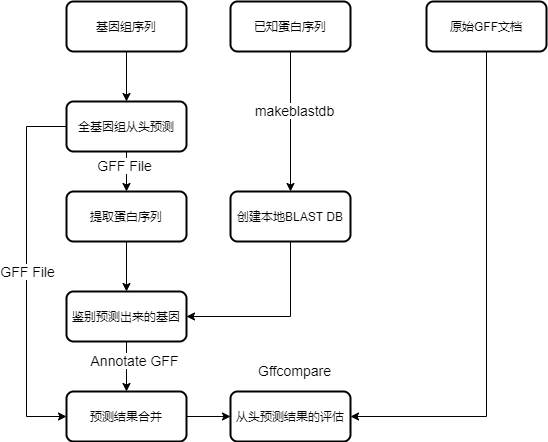
\includegraphics[scale=0.65]{figs/flowchart.drawio.png}
\caption{实验流程图}
\label{fig:任务流程图}
\end{figure}

\begin{outline}[enumerate]
 \1 于GenBank数据库选择与下载下列物种的基因组序列和注释文档
   \2 Saccharomyces cerevisiae
   \2 Caenorhabditis elegans
   \2 Paramecium tetraurelia
 \1 于UniprotKB数据库下载这些物种所在分类的所有已知蛋白(排除该物种自身的已知蛋白)
 \1 基因预测软件:安排两人对Augustus等软件检索相关的评测比较的文章,并选取若干个工具,安装使用测试,解决软件使用过程中出现的问题
 \1 使用上一步选定的多个基因预测软件,对全基因组序列进行基因预测和结构建模,结果转成GFF3格式
 \1 利用gffcompare软件比较不同软件的预测结果,进行挑选与整合
    \2 解读gffcompare结果
    \2  两两共同特征的选择: e.g. 局部重合,完全重合
    \2 而后进行挑选与整合
 \1 将4和5的结果与1下载的原始注释文档进行比对,分析异同,评估优劣,改良
 \1 本地blast配置,用blast比对鉴别第4和5步的结果中输出的蛋白质
 \1 用blast92gff3.pl程序转化blast结果为gff3格式(修改参数)
 \1 利用JBrowse和IGV将注释组的注释信息可视化,比较两者优劣
\end{outline}
   
\subsubsection{任务分工}

\begin{itemize}
    \item [1,2]:张书凡
    \item [3,4]:裘\yu 然,郑宇翔
    \item [5,]:李定洋,朱泽峰
    \item [6,]:朱泽峰,张书凡
    \item [7,8]:李定洋
    \item [9,]:张书凡
\end{itemize}

\section{软硬件}

操作系统与运行环境等参数

\begin{outline}[enumerate]
\1 操作平台:阿里云服务器
\1 平台配置:双核2.40GHz CPU,4GiB内存
\1 操作系统:Ubuntu 20.04 (64bit)
\1 使用软件:
    \2 Augustus 3.3
    \2 GeneMark-ES ver 4.*
    \2 Geneid 1.2
    \2 Gffread
\1 编程语言
    \2 Python3
    \2 Perl
    \2 R
    \2 Shell Script
\end{outline}


\section{实验步骤与结果}

\subsection{GenBank数据库选择与下载选定物种的基因组序列和注释文档 (by 张书凡)}

从NCBI的Genome数据库下载草履虫、秀丽线虫、酵母菌的基因组序列和GFF格式的注释信息,选择下载的具体物种编号如下:

\begin{outline}[enumerate]
\1 酿酒酵母
\2 Saccharomyces cerevisiae S288C (assembly R64)
\1 秀丽线虫
\2 Caenorhabditis elegans (assembly WBcel235)
\1 草履虫
\2 Paramecium tetraurelia (assembly ASM16542v1)
\end{outline}


\subsection{UniprotKB数据库下载选定物种所在分类的所有已知蛋白 (by 张书凡)}

从UniPort数据库下载下面三个物种所在分类的所有已知蛋白(排除该物种自身的已知蛋白质)。草履虫属于纤毛亚门,秀丽线虫属于线虫门,酵母菌属于真菌界。搜索关键词如下:

\begin{outline}[enumerate]
\1 酵母:`taxonomy:fungi NOT "saccharomyces cerevisiae" AND reviewed:yes`
\1 线虫:`taxonomy:nematoda NOT "caenorhabditis elegans" AND reviewed:yes
\1 草履虫:`taxonomy:ciliophora NOT "paramecium tetraurelia" AND reviewed:yes`
\end{outline}

\begin{minipage}{\linewidth}
\centering
\captionof{table}{UniprotKB搜索结果统计} \label{tab:title} 
\begin{tabular}{ C{1.25in} C{1.85in} C{1.85in}}\toprule[1.5pt]
\textbf{物种} & \textbf{搜索到的近缘
物种已知蛋白数量}\\ \hline
酿酒酵母 & 25522 \\ 
秀丽线虫 & 836\\ 
草履虫 & 271\\ 
\bottomrule[1.25pt]
\end {tabular}\par
\bigskip
\end{minipage}

\subsection{全基因组序列的基因从头预测与结构建模结果解析 (by 裘yu然,郑宇翔)}

选定如下软件的理由参见上述。

在其他小组成员分别利用Augustus,Geneid,GeneMark三个物种的基因组数据进行分析后,得到了软件输出的GFF与GTF格式文件。预先设定的分析流程是按照Augustus的GFF输出文件内容来安排,即提取其中的蛋白序列信息于建立好的blast数据库进行搜索,找到对应的UniProt条目进而重注释例如Augustus输出的结果,方便后续进行对比分析。但是在实际实验过程中发现,Geneid,GeneMark最新版本输出结果中(GFF3格式或GTF格式文件)没有所需的蛋白序列信息。因此安排负责同学对软件参数与版本进行调查,最终决定回退至特定版本,以获得序列信息。(by 朱泽峰)


Augustus的最终预测结果基因数目如下(by裘\yu 然):

\begin{minipage}{\linewidth}
\centering
\captionof{table}{Augustus最终预测结果基因数目} \label{tab:title} 
\begin{tabular}{ C{1.25in} C{.85in} *4{C{.75in}}}\toprule[1.5pt]
\textbf{物种}                                                        & 酵母菌  & 秀丽线虫 & 草履虫   \\ \hline
\textbf{\begin{tabular}[c]{@{}c@{}}Augustus\\ 预测基因数目\end{tabular}} & 5465 & 6445 & 12983 \\ 
\bottomrule[1.25pt]
\end {tabular}\par
\bigskip
\end{minipage}

GeneMark-ES对于三个物种的基因预测量分别如下(by裘\yu 然):

\begin{minipage}{\linewidth}
\centering
\captionof{table}{GeneMark-ES最终预测结果基因数目} \label{tab:title} 
\begin{tabular}{ C{1.25in} C{.85in} *4{C{.75in}}}\toprule[1.5pt]
\textbf{物种}                                                    & 酵母菌  & 秀丽线虫  & 草履虫   \\ \hline
\textbf{\begin{tabular}[c]{@{}c@{}}GMES\\ 预测基因数目\end{tabular}} & 5471 & 22591 & 13800 \\ 
\bottomrule[1.25pt]
\end {tabular}\par
\bigskip
\end{minipage}


Geneid预测得到的基因数量如下所示(by郑宇翔):

\begin{minipage}{\linewidth}
\centering
\captionof{table}{Geneid最终预测结果基因数目} \label{tab:title} 
\begin{tabular}{ C{1.25in} C{.85in} *4{C{.75in}}}\toprule[1.5pt]
\textbf{物种}                                                    & 酵母菌  & 秀丽线虫  & 草履虫   \\ \hline
\textbf{\begin{tabular}[c]{@{}c@{}}Geneid\\ 预测基因数目\end{tabular}} & 4073 & 5705 & 23386 \\
\bottomrule[1.25pt]
\end {tabular}\par
\bigskip
\end{minipage}

根据目前的研究结果,酿酒酵母共有6275个基因,其中可能约有5800个真正具有功能;秀丽隐杆线虫有大约20000个基因;而草履虫有大约4万个基因。Augustus的酵母预测结果较为准确,但其余两个物种的结果则相差较远;GeneMark的对于线虫和酵母的预测结果较好,但是草履虫依然较低;Geneid只预测出了4073个酵母的基因,结果远少于实际情况,这可能是因为提供的模型只考虑TGA作为终止密码子所致,而Geneid对于草履虫的预测则较为准确。这表明了不同基因预测软件对于不同物种的适用程度是不同的。

注:3.3版本的augustus中没有包含草履虫的模型,在从头预测草履虫的基因时使用了草履虫的近缘物种——四膜虫的模型进行预测。在geneid中,酿酒酵母(Saccharomyces cerevisiae)使用的是日本裂殖酵母(Schizosaccharomyces japonicus)的配置文件。草履虫的配置文件只考虑TGA作为终止密码子。
这些都可能会对运行结果产生影响

\subsection{不同软件预测结果的比较、挑选与整合(by 李定洋、朱泽峰)}

利用gffcompare比较不同软件之间的预测结果,进行挑选与整合,此步骤有如下要点:

\begin{itemize}
    \item 解读.stats文件结果
    \item 解读.combined.gtf文件结果
    \item 对加入-R参数(要求完全重合)与未加入-R参数(允许局部重合)的结果进行对比
    \item 两两共同特征的选择,而后进行挑选与整合
\end{itemize}

进行不同软件间结果的对比,对于某一特定物种,依次取各个软件的结果作为参考GFF,且分别产出只考虑完全覆盖或反者的结果。对于同时得到的conbined.gff文件,鉴于我们是提供多个输入GTF/GFF文件得到的,其中包含每个样本中所有注释的并集。\citep{pmid32489650}

利用python脚本对.stats文件内容进行提取得到表格示例如下表:

\begin{minipage}{\linewidth}
\centering
\captionof{table}{stats文件信息提取} \label{tab:title} 
\begin{tabular}{ C{0.55in} *6{C{0.75in}}}\toprule[1.5pt]
\textbf{level} & \textbf{Sensitivity} & \textbf{Precision} & \textbf{ref}               & \textbf{fileName} & \textbf{to}              & \textbf{fileGroup} \\ \hline
Base level     & 74.2                 & 27.9               & ele\_augustus & AU\_ELE     & ele\_genid & AU\_ELE            \\
Exon level     & 64.3                 & 19.3               & ele\_augustus & AU\_ELE     & ele\_genid & AU\_ELE            \\
Intron level   & 75.6                 & 23.1               & ele\_augustus & AU\_ELE     & ele\_genid & AU\_ELE            \\
...            & ...                  & ...                & ...                        & ...               & ...                      & ...                \\
Base level     & 99.0                 & 99.3               & Sac\_cerevisiae        & SC\_R       & Sc\_gmes            & SC                 \\
\bottomrule[1.25pt]
\end {tabular}\par
\bigskip
\end{minipage}


从结果看到,以Augustus预测文件为参考GFF的结果在各个物种中普遍较差,而以GeneMark-ES或Geneid为参考GFF的结果的非Augustus相关的BaseLevel与ExonLevel相对较好。且值得注意,要求完全重合的结果与允许局部重合结果在评估上,于Sensitivity水平上都有些许提升,但是Precision无明显变化,这表明丢弃局部重合的结果后,各软件预测的结果更为符合参考GFF所标记的基因。但是值得指出的是上述情况中,草履虫的预测结果始终是最差的。

鉴于Augustus的结果作为参考GFF的结果较差有些出乎意料,选择特定软件的为参考的combined gff步骤置于下面步骤进行(即两两共同特征的选择,而后进行挑选与整合步骤)。

\subsection{各软件原始预测结果及整合预测结果与原GFF文件进行对比、分析异同、评估优劣与改良 (by 朱泽峰)}

分别设定各个物种的参考GFF文件以及各个软件的对应GFF结果文件,运行gffcompare。

\begin{figure}[htbp]
\centering
\subfigure[Augustus结果对比]{
\includegraphics[width=10cm]{figs/tab_au_1.png}
%\caption{fig1}
}
\quad
\subfigure[GMES结果对比]{
\includegraphics[width=10cm]{figs/tab_gmes_1.png}
}
\quad
\subfigure[Geneid结果对比]{
\includegraphics[width=10cm]{figs/tab_geneid_1.png}
}
\caption{不同软件结果与原始GFF对比}
\end{figure}

可以看到:

\begin{itemize}
    \item 对于Saccharomyces cerevisiae,除去内含子层面的预测,Augustus在Precision层面(即给出的预测结果的正确率)以及Sensitivity层面(即正确预测出的结果于参考GFF中的占比)的预测都足够理想
    \item 对于Caenorhabditis elegans,在Sensitivity层面的预测不够良好,即正确预测出的结果于参考GFF中的占比较低,且转录本层面的Precision也不够理想
    \item 对于Paramecium tetraurelia,仅BaseLevel的Precision数值较高,其余数值都很低,说明Augustus选用的模型对于本次实验的数据材料存在比较明显的错配
\end{itemize}

对于某一特定物种,分别把某一软件输出结果作为参考GFF的conbinded gff文档与原始GFF文档进行对比,以此与上述软件原输出的预测结果效果进行对比可以发现:

\begin{itemize}
    \item 对于酿酒酵母,于BaseLevel上的预测都较高,且注意到整合后相比于原始结果,precision都降低,但是sencisity升高
    \item 对于秀丽线虫和草履虫,Augustus以为参考的整合GFF效果最差,GMES最好,Geneid次之
    \item 对于草履虫,Geneid的Sensitivity明显较好
\end{itemize}

因此可以总结到,对于酿酒酵母,单纯用Augustus的预测结果最佳;对于秀丽线虫,以GeneMark-ES为预测结果为参考并整合Geneid、Augustus的结果最佳;对于草履虫,以Geneid的预测结果为参考并整合GeneMark-ES、Augustus的结果最佳。



\subsection{预测结果的序列提取(by 张书凡)}

对4中Augustus工具得到的三个gff3文件,使用sed命令能够便捷提取其中的蛋白质序列;对4中geneid得到的三个物种的geneid格式文件,使用脚本fetch.py提取其中的蛋白质序列;GMES的序列有软件输出方提供。

向GenMark与geneid工具得出的预测结果中添加匹配上的蛋白质ID的方法与Augustus一致。由于不同预测软件给出的gff文件略有不同,添加蛋白ID的脚本也因此略有不同。

\subsection{本地BLAST数据库的创建与同源基因搜索做格式转换(by李定洋)}

使用 makeblastdb 程序,对上述 FASTA 格式的蛋白序列进行处理,建立本地 BLAST 数据库。并使用 blastp 程序,把各软件预测的蛋白质序列和上述建立的本地 BLAST 数据库进行比对。此过程进行的较为顺利,无意外情况。同时进行匹配蛋白数量的统计:

\begin{minipage}{\linewidth}
\centering
\captionof{table}{Blast比对结果统计} \label{tab:title} 
\begin{tabular}{ *4{C{1.15in}}}\toprule[1.5pt]
\textbf{鉴别出来各物种的蛋白数量} & \textbf{酵母(原始基因数量6445)} & \textbf{线虫(原始基因数量47632)} & \textbf{草履虫(原始基因数量39581)}\\ \hline
Augustus                         & 4483 & 1213 & 1484 \\
Genemark & 4442 & 4452 & 1317 \\
Geneid   & 4066 & 4146 & 147\\
\bottomrule[1.25pt]
\end {tabular}\par
\bigskip
\end{minipage}

使用 blast92gff3.pl程序,把结果转成 GFF3 格式。

\subsection{JBrowse和IGV的注释信息可视化及比较(by张书凡)}

\begin{figure}[htbp]
\centering
\subfigure[导入文件类型的比较1]{
\includegraphics[width=7cm]{figs/genomics_lab1_fig5.png}
}
\quad
\subfigure[导入文件类型的比较2]{
\includegraphics[width=7cm]{figs/genomics_lab1_fig6.png}
}
\quad
\subfigure[IGV可视化]{
\includegraphics[width=7cm]{figs/genomics_lab1_fig7.png}
}
\quad
\subfigure[JBrowse可视化]{
\includegraphics[width=7cm]{figs/genomics_lab1_fig8.png}
}
\caption{不同软件结果与原始GFF对比}
\end{figure}

\begin{outline}[enumerate]
\1 JBrowse与IVG安装上的比较
\2 JBrowse与IVG支持所有的操作系统,均可以安装,且有详细的安装教程。JBrowse与IVG均提供本地app以及嵌入web的app。从安装的方面,这两个工具都很便利。IVG的优势是他提供了在线的web服务,无需安装直接使用,网址如下:https://igv.org/app/
\1 从JBrowse与IVG支持的导入文件类型的比较
\2 IVG支持的文件类型相比JBrowse更多,同时自带下载默认的参考基因组
\2 图4来自“Which genome browser to use for my data ?”这篇report是2019.7发表的,从多个方面比较目前主流的genome browser,后续比较的参考基本上都是来源于该文章
\2 reference: https://wikis.univ-lille.fr/bilille/genome_browser

\1 从JBrowse与IVG可视化和使用便利性的角度比较
\2 用户界面方面,JBrowse相对要更加美观一些,IGV显得比较陈旧。使用方面,IGV提供了额外的操作,包括:按照基因ID搜索片段、调节轨道高度、颜色、注释字体大小等。这里的总结就是JBrowse更美观,而IVG更加功能强大丰富
\1 JBrowse还有一点比较突出的就是对注释信息的整体特别好,单独弹出了页面方便复制信息。此外很重要一点的是JBrowse会根据导入的基因组序列文件以及gff注释文件的信息(基因的位置信息),给出每一个基因的序列
\end{outline}

\begin{figure}[h!]
\centering
\includegraphics[scale=0.65]{figs/genomics_lab1_fig4.png}
\caption{JBrowse注释信息整体性}
\end{figure}

\newpage

\bibliographystyle{plain}
\bibliography{references}
\end{document}